\documentclass{article}
\usepackage{cite}
\usepackage{amsmath,amssymb,amsfonts}
\usepackage{algorithmic}
\usepackage{graphicx}
\usepackage{textcomp}
\usepackage{hhline}
\usepackage[acronym]{glossaries}
\usepackage{amssymb}
\usepackage{graphicx}
\usepackage{multirow}
\usepackage{hhline}
\usepackage{ctable}
\usepackage{float}
\usepackage{color}


\title{Experimental Results}
\begin{document}
   \maketitle

\section{Effect of simulation fixed step size on the accuracy, architecture  on neural network replacement of PID in dc motor speed control \label{step_size}}
\subsection{Performance with 10 hidden neurons}
Training Parameter: Tansig hidden layer, maximum epoch 150, stopping criteria epoch, minimum gradient, only the maximum epoch is changed everything else stays default. Such as input Delays = 1:2;
feedback Delays = 1:2; hidden Layer Size = 10; 
With smaller step size, we have more data, and less error. Worst performance is shown in bold
\begin{table}[H]
\centering
\caption{\label{tab1}Effect of Fixed step size on Accuracy Testing Accuracy - Hidden Neurons 10}
\begin{tabular}{|l|l|l|}
\hline
Fixed Step Size & Training Error & Test Error \\ \hline
0.001           & 2.4116e-06     & 1.9052e-06 \\ \hline
0.01            & 2.3287e-06     & 1.8463e-06 \\ \hline
0.1             & 7.4570e-05     & 6.1457e-05 \\ \hline
0.2             & \textbf{2.8739e-04}     & \textbf{3.4440e-04} \\ \hline
\end{tabular}
\end{table}
\subsection{Performance with 3 hidden neurons}
\begin{table}[H]
\centering
\caption{\label{tab2}Effect of Fixed step size on Testing Accuracy - Hidden Neurons 3}
\begin{tabular}{|l|l|l|}
\hline
Fixed Step Size & Training Error & Test Error \\ \hline
0.001           & 2.5779e-06     & 2.0565e-06 \\ \hline
0.01            & 2.5016e-06     & 1.9960e-06 \\ \hline
0.1             & 9.5324e-05     & 7.7856e-05 \\ \hline
0.2             & \textbf{3.6994e-04 }     & \textbf{4.0580e-04} \\ \hline
\end{tabular}
\end{table}
From the experiment we can conclude that a fixed step size of 0.01 will give better performance and the minimum allowed number of neurons in the hidden layer is 3.

\section{Effect of Delay on the accuracy of neural network replacement of PID in DC motor speed control}
Using the fixed step size obtained in \ref{step_size}, and the minimum hidden layer of 3 neurons, the following are the results for varying the delay. All other parameters are kept constant.
\begin{table}[H]
\centering
\caption{\label{tab3}Effect of Delay on  Testing Accuracy}
\begin{tabular}{|l|l|l|}
\hline
Delay & Training Error & Test Error \\ \hline
2     & 2.5016e-06     & 1.9960e-06 \\ \hline
3     & 2.5152e-06     & 2.0026e-06 \\ \hline
6     & 2.4874e-06     & 1.9868e-06 \\ \hline
9     & 2.4872e-06     & 1.9871e-06 \\ \hline
12    & 2.4856e-06     & 1.9859e-06 \\ \hline
\end{tabular}
\end{table}
Observation: as the delay increases, the test accuracy gets better even though the difference is really small. However, the higher the value of the network delay, the more "complex" the architecture.

\section{Effect of Hidden Neurons on the Performance of Activation Functions}
\begin{itemize}
\item With each AF, does the number of hidden neurons have effect on their performance?
\item How low can we go before the error is unacceptable?
\item Which AF gives the minimum epoch,error with hidden neuron settings.
\end{itemize}
\begin{table}
\centering
\caption{\label{tab3}Effect of Activation Function on  Testing Accuracy}
\begin{tabular}{|l|l|l|l|l|l|l|}
\hline
\begin{tabular}[c]{@{}l@{}}Number of\\  Neurons\end{tabular} & \multicolumn{2}{l|}{3}                                        & \multicolumn{2}{l|}{4}                                        & \multicolumn{2}{l|}{10}                                      \\ \hline
Function                                                     & Epoch  & \begin{tabular}[c]{@{}l@{}}Test\\ Error\end{tabular} & Epoch  & \begin{tabular}[c]{@{}l@{}}Test\\ Error\end{tabular} & Epoch & \begin{tabular}[c]{@{}l@{}}Test\\ Error\end{tabular} \\ \hline
ElliotSig                                                    & 800    & 2.0010e-04                                           & 800    & 2.0004e-04                                           &       &                                                      \\ \hline
SQNL                                                         & 761.69 & 1.9967e-04                                           & 776.47 & 1.9951e-04                                           &       &                                                      \\ \hline
TanSig                                                       & 799.8  & 1.9968e-04                                           & 800    & 1.9921e-04                                           &       &                                                      \\ \hline
ReLu                                                         & 124.35 & 4.5861e-04                                           & 132.23 & 3.7159e-04                                           &       &                                                      \\ \hline
SQLU                                                         & 674.57 & 2.0031e-04                                           & 771.14 & 2.0023e-04                                           &       &                                                      \\ \hline
ELU                                                          & 681.81 & 2.0030e-04                                           & 776.21 & 2.0021e-04                                           &       &                                                      \\ \hline
Leaky ReLu                                                   & 132.06 & 3.2981e-04                                           & 128.06 & 3.7556e-04                                           &       &                                                      \\ \hline
\end{tabular}
\end{table}


\section{Write Up}
The use of PID as a controller in control system applications is ubiquitous. Although the theory behind PID is really simple but the design and implementation of PID controllers are known to be time consuming and difficult. Moreover, PID are linear systems and can only learn a particular plant based on their predefined settings. NN on the other hand are characterised with learning opportunities and adaptability in nature. This means that a NN based controller is robust to several input types and even maybe different plant architectures as will be proved in this work.

\section{Neural Network Replacement of PID}
We further demonstrated the ability of the proposed SQNL on control application. The use of PID for controlling control systems is a wide area of study however, in recent years, the disadvantages of PID controller have being solved by Neural Network Controllers. We therefore replaced the PID controller with 3 hidden neuron Neural Network architecture using the illustration in 


\begin{figure}
\centering
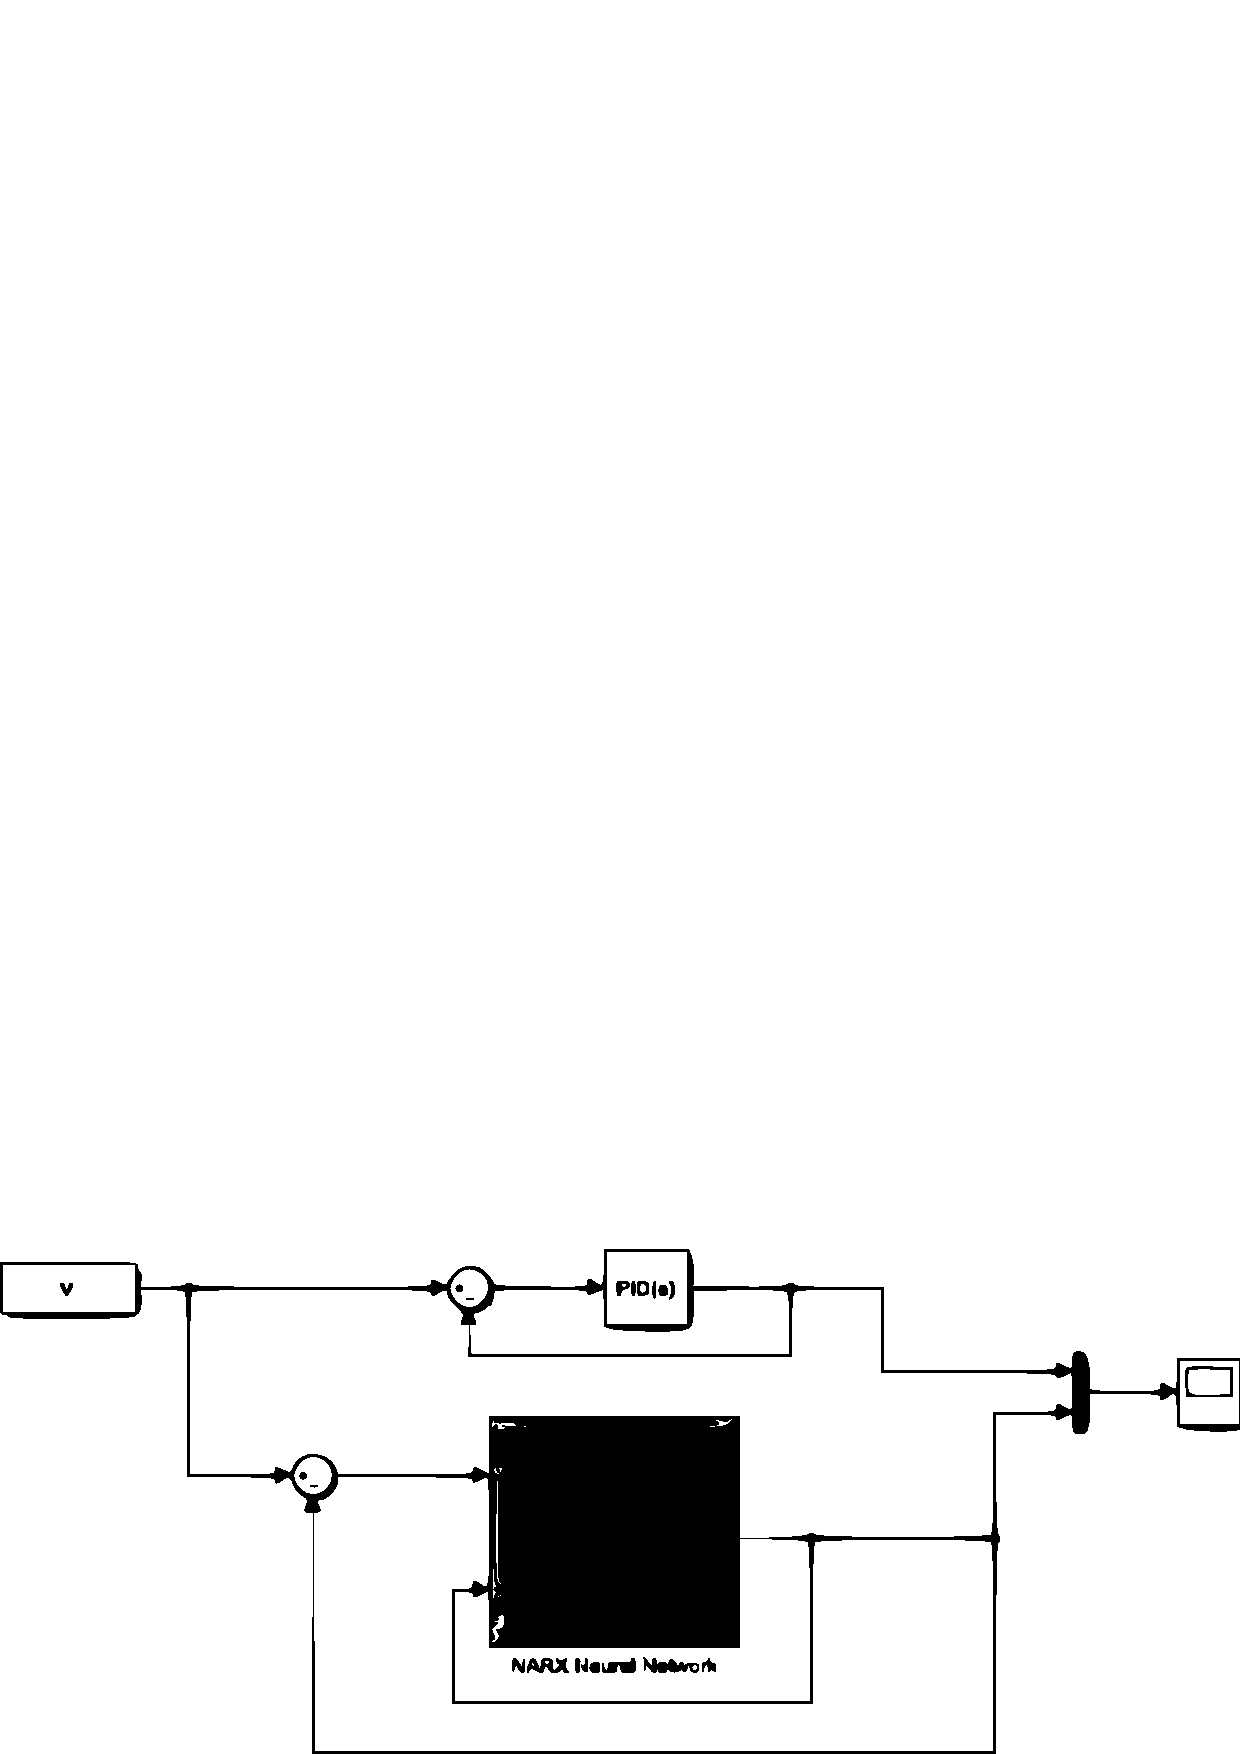
\includegraphics[scale=0.65]{PID_NN.jpg}
\caption{\label{fig:compare_rbf} The Experimental setup of the NN replacement of PID controller}
\end{figure}

\end{document}